%% This file is a portion of the source for Revised Edition 1.1 of
%% Operating Systems and Middleware: Supporting Controlled
%% Interaction, Copyright 2011 by Max Hailperin.  This work is
%% licensed under the Creative Commons Attribution-ShareAlike 3.0
%% Unported License. To view a copy of this license, visit
%% http://creativecommons.org/licenses/by-sa/3.0/ or send a letter to
%% Creative Commons, 171 Second Street, Suite 300, San Francisco,
%% California, 94105, USA.
\chapter{Atomic Transactions}
\label{transactions-chapter}
\section{Introduction}

In Chapter~\ref{synchronization-chapter}, I described mutual exclusion as a mechanism
for ensuring that an object undergoes a sequence of
invariant-preserving transformations and hence is left in a state
where the invariant holds.  (Such states are called
\vocab{consistent} states.)  In particular, this was the idea behind
monitors.  Any monitor object is constructed in a consistent state.
Any public operation on the monitor object will work correctly when
invoked in a consistent state and will reestablish the invariant
before returning.  No interleaving of actions from different monitor
operations is allowed, so the monitor's state advances from one
consistent state to the next.

In this chapter, I will continue on the same theme of
invariant-preserving state transformations.  This time through,
though, I will address two issues I ignored in
Chapter~\ref{synchronization-chapter}:
\begin{enumerate}
\item
Some invariants span multiple objects; rather than transforming a
single object from a consistent state to another consistent state, you may
need to transform a whole system of objects from one consistent state
to the next.  For example, suppose you use objects to form a rooted
tree, with each object knowing its parent and its children, as shown
in Figure~\ref{scan-5-1}.
\begin{figure}
\centerline{\includegraphics{hail_f0501}}
%\centerline{\epsfbox{scan-5-1.eps}}
\caption{Rooted trees with pointers to children and parents: (a)
  example satisfying the invariant; (b) invariant violated because
  E's parent is now C, but E is still a child of D and not of C;
  (c) invariant restored because the only child pointer leading to E
  again agrees with E's parent pointer.  The complete transformation
  from Part (a) to Part (c) requires modifications to nodes C, D, and E.}
\label{scan-5-1}
\end{figure}
An
invariant is that X has Y as a child if and only if Y has X as its
parent.  An operation to move a node to a new position in the tree
would need to change three objects (the node, the old parent, and the
new parent) in order to preserve the invariant.
\item
Under exceptional circumstances an operation may \vocab{fail}, that is,
be forced to give up after doing only part of its invariant-preserving
transformation.  For example, some necessary resource may be
unavailable, the user may press a Cancel button, the input may fail a
validity check, or a hardware failure may occur.  Nonetheless, the
system should be left in a consistent state.
\end{enumerate}

An \foldvocab{atomic}{transaction} is an operation that takes a system
from an observable initial state to an observable final state, without
any intermediate states being observable or perturbable by other
atomic transactions.  If a system starts with a consistent initial
state and modifies that state using only invariant-preserving
atomic transactions, the state will remain consistent.
Atomicity\index{atomic} must be preserved in the face of both
concurrency and failures.  That is, no transaction may interact with a
concurrently running transaction nor may any transaction see an
intermediate state left behind by a failed transaction.  The former
requirement is known as \vocab{isolation}.  The latter requirement
lacks a generally agreed-upon name; I will call it \vocab{failure atomicity}.

Often, atomic transactions are simply called \vocabs{transaction}.  In
fact, according to many authors, atomicity is part of the definition
of a transaction.  Unfortunately, there are other authors for whom
transactions need not be atomic.  Because of this lack of agreement on
the nomenclature, I have introduced this chapter with the full phrase
``atomic transactions'' to make my focus clear.  Henceforth, I will
skip the modifier ``atomic'' and use only ``transactions,'' with the
understanding that they are atomic unless otherwise specified.

Many transaction systems require not only atomicity, but also
\vocabindex{durability}{durable}.  A transaction is durable if the
state of a successfully completed transaction remains intact, even if
the system crashes afterward and has to be rebooted.  Each successful
transaction ends with an explicit \vocab{commit} action, which
signifies that the consistent final state has been established and
should be made visible to other transactions.  With durable
transactions, if the system crashes after the commit action, the final
transformed state will be intact after system restart.  If the crash
occurs before the commit action, the system will be back in the
initial, unchanged state after restart.

Note that failure atomicity is slightly simpler for nondurable
transactions.  Atomicity across system crashes and restarts is easy to
arrange: by clearing all memory on restart, you can guarantee that no
partially updated state is visible after the restart---no updates at
all, partial or otherwise, will remain.  This clearing of memory will
happen automatically if the computer's main semiconductor DRAM memory
is used, because that memory is \vocab{volatile}, that is, it does not
survive reboots.  (Strictly speaking, volatility means the memory does
not survive a loss of power; reboots with the power left on generally
clear volatile memory as well, however.)

Even nondurable transactions must ensure failure atomicity
for less dramatic failures in which the system is not rebooted.  For
example, a transaction might do some updates, then discover invalid
input and respond by bailing out.
To take another example, recovering from a
detected deadlock might entail aborting one of the deadlocked
transactions.  Both situations can be handled using an
explicit \vocab{abort} action, which indicates the transaction should
be terminated with no visible change made to the state.  Any changes
already made must be concealed, by undoing them.

In 1983, \index{Harder, Theo@H{\"a}rder, Theo}H{\"a}rder and
\index{Reuter, Andreas}Reuter coined a catchy phrase by saying that
whether a system supports transactions is ``the \index{ACID}ACID test of the
system's quality.''  The ACID acronym indicates that transactions are
\vocab{atomic}, \vocab{consistent}, \vocab{isolated}, and
\vocab{durable}.  This acronym is quite popular, but somewhat
redundant.  As you have seen, a transaction system really only provides
two properties: atomicity and durability.  Consistency is a property
of system states---a state is consistent if the invariants hold.
Transactions that are written correctly (so each preserves invariants)
will leave the state consistent if they execute atomically.  Isolation
simply is another name for atomicity in the face of concurrency:
concurrent transactions must not interact.

The properties of atomicity and durability refer to transactions,
independent of the objects on which the transactions operate.
Returning to the earlier rooted tree example of moving a node to a new
position, a transaction might modify the node, the old parent, and the
new parent, all within one atomic unit.  This stands in contrast
to monitors, each of which controls a single
object.

To obtain the requisite atomicity with monitors, the whole tree could
be a single monitor object, instead of having one monitor per node.  The tree
monitor would
have an operation to move one of its nodes.  In general, this approach
is difficult to reconcile with modularity. Moreover, lumping lots of
data into one monitor creates a performance problem.  Making the
whole system (or a large chunk of it) into one monitor would prevent
any concurrency.  Yet it ought to be possible to concurrently move two
nodes in different parts of a tree.  Atomic transactions allow
concurrency of this sort while still protecting the entire
transformation of the system's state.

This point is worth emphasizing.  Although the system's state remains
consistent \emph{as though} only one transaction were executed at a
time, transactions in fact execute concurrently, for performance
reasons.  The transaction system is responsible for maintaining
atomicity in the face of concurrency.  That is, it must ensure that
transactions don't interact with one another, even when running
concurrently.  Often the system will achieve this isolation by
ensuring that no transaction reads from any data object being
modified by another transaction.  Enforcing this restriction entails introducing
synchronization that limits, but does not completely eliminate, the
concurrency.

In Section~\ref{trasactions-examples-section}, I will sketch several examples of the ways in
which transactions are used by middleware and operating systems to
support application programs.  Thereafter, I present techniques used
to make transactions work, divided into three sections.  First, Section~\ref{atomicity-mechanisms-section}
explains basic techniques for ensuring the atomicity of transactions,
without addressing durability.  Second, Section~\ref{wal} explains how
the mechanism used to ensure failure atomicity can be extended to also
support durability.  Third,
Section~\ref{additional-transaction-mechanisms-section} explains a few additional mechanisms
to provide increased concurrency and
coordinate multiple participants cooperating on a single transaction.
Finally, Section~\ref{security-and-transactions-section} is devoted to security issues.
The chapter concludes with exercises, exploration and programming projects, and notes.

\section{Example Applications of Transactions}\label{trasactions-examples-section}

The transaction concept is much more pervasive in middleware than in
operating systems.  Therefore, of the three examples presented in the
following subsections, the first two are from middleware systems.
Sections \ref{db-transaction-section} and
\ref{transactions-message-queuing-systems-section} explain the two
most long-standing middleware applications, namely database systems
and message-queuing systems.
Moving into the operating systems arena, Section~\ref{jfs-transactions-section} 
explains the role that transactions play in
journaled file systems, which are the current dominant form of file
system.

\subsection{Database Systems}\label{db-transaction-section}

The transaction concept is most strongly rooted in \vocabs{database
system}; for decades, every serious database system has provided
transactions as a service to application programmers.  Database
systems are an extremely important form of middleware, used in almost
every enterprise information system.  Like all middleware,
database systems are built on top of operating system services, rather
than raw hardware, while providing  general-purpose services
to application software.  Some of those services are synchronization
services: just as an operating system provides mutexes, a database
system provides transactions.

On the other hand, transaction services are not the central, defining
mission of a database system.  Instead, database systems are primarily
concerned with providing persistent data storage and convenient means
for accessing the stored data.  Nonetheless, my goal in this chapter is to show how transactions fit
into relational database systems.  I will cover just enough of the SQL
language used by such systems to enable you to try out the example on
a real system.  In particular, I show the example using the Oracle
database system.

Relational database systems manipulate tables of data.  In Chapter~\ref{synchronization-chapter}'s
discussion of deadlock detection, I showed a
simple example from the Oracle database system involving two
accounts with account numbers 1 and 2.  The scenario
(as shown in Figure~\ref{oracle-deadlock} on
page~\pageref{oracle-deadlock}) involved transferring money from each
account to the other, by updating the balance of each account.  Thus,
that example involved a table called \verb|accounts| with two columns,
\verb|account_number| and \verb|balance|.  That table can be created
with the SQL command shown here:
\begin{verbatim}
create table accounts (
  account_number int primary key,
  balance int);
\end{verbatim}
Similarly, you can initialize account~1 to \$750 and account~2 to
\$2250 by using the following commands:
\begin{verbatim}
insert into accounts values (1, 750);
insert into accounts values (2, 2250);
\end{verbatim}
At this point, you can look at the table with the \verb|select| command:
\begin{verbatim}
select * from accounts;
\end{verbatim}
and get the following reply:
\begin{verbatim}
ACCOUNT_NUMBER    BALANCE                                                       
-------------- ----------                                                       
             1        750                                                       
             2       2250                                                       
\end{verbatim}
(If you are using a relational database other than Oracle, the format
of the table may be slightly different.  Of course, other aspects of
the example may differ as well, particularly the deadlock detection
response.)

At this point, to replicate the deadlock detection example from
Figure~\ref{oracle-deadlock}, you will need to open up two different
sessions connected to the database, each in its own window.  In the
first session, you can debit \$100 from account~1, and in the second
session you can debit \$250 from account~2.  (See
page~\pageref{oracle-deadlock} for the specific SQL commands.)  Now
in session one, try to credit the \$100 into account~2; this is blocked,
because the other session has locked account~2.  Similarly, session two
is blocked trying to credit its \$250 into account~1, creating a
deadlock, as illustrated in Figure~\ref{scan-5-2}.
\begin{figure}
\centerline{\includegraphics{hail_f0502}}
%\centerline{\epsfysize=5in\epsfbox{scan-5-2.eps}}
\caption{Two transfer transactions deadlock when each waits for
  exclusive access to the account for which the other already has
  obtained exclusive access.  In this diagram, the vertical dimension
  represents the passage of time.}
\label{scan-5-2}
\end{figure}
As you saw, Oracle detects the deadlock and chooses to cause
session one's update request to fail.

Having made it through all this prerequisite setup, you are in a
position to see the role that transactions play in situations such as
this.  Each of the two sessions is processing its own transaction.
Recall that session one has already debited \$100 from account~1 but
finds itself unable to credit the \$100 into account~2.  The
transaction cannot make forward progress, but on the other hand, you
don't want it to just stop dead in its tracks either.  Stopping would block the
progress of session two's transaction.  Session one also cannot just bail
out without any cleanup: it has already debited \$100 from account~1.
Debiting the source account without crediting the destination account
would violate atomicity and make customers angry besides.

Therefore, session one needs to abort its transaction, using the
\verb|rollback| command.  Aborting will back out of the transaction's earlier debiting
of \$100 from account~1 and release its lock on that account.  As a
result, session two's attempt to credit \$250 into account~1 can
finally stop hanging and complete.  Continuing my earlier tradition
of showing session one at the left margin and session two indented
four spaces, the interaction would look like:
\begin{verbatim}
SQL> rollback;

Rollback complete.

    1 row updated.
\end{verbatim}

Of course, whoever was trying to transfer \$100 from account~1 to
account~2 still wants to do so.  Therefore, after aborting that
transaction, you should retry it:
\begin{verbatim}
SQL> update accounts set balance = balance - 100
                     where account_number = 1;
\end{verbatim}
This command will hang, because session two's transaction now has both
accounts locked.  However, that transaction has nothing more it needs
to do, so it can commit, allowing session one to continue with its retry:
\begin{verbatim}
    SQL> commit;

    Commit complete.

1 row updated.

SQL> update accounts set balance = balance + 100 
                     where account_number = 2;

1 row updated.

SQL> commit;

Commit complete.

SQL> select * from accounts;

ACCOUNT_NUMBER    BALANCE                                                       
-------------- ----------                                                       
             1        900                                                       
             2       2100                                                       
\end{verbatim}
Notice that at the end, the two accounts have been updated correctly.
For example, account~1 does not look as though \$100 was debited from
it twice---the debiting done in the aborted transaction was wiped
away.  Figure~\ref{scan-5-3} illustrates how the transactions recover
from the deadlock.
\begin{figure}
\centerline{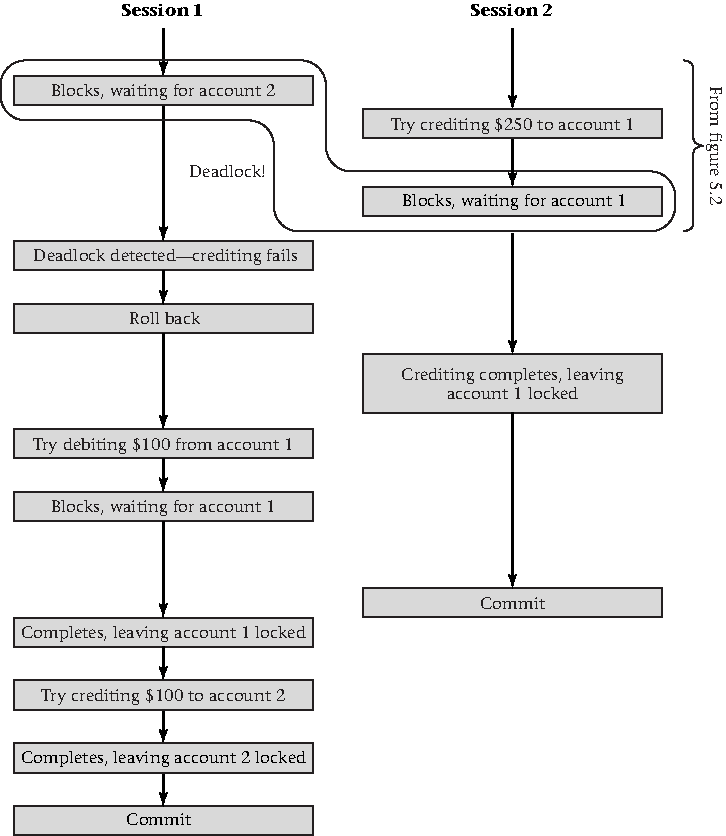
\includegraphics{hail_f0503}}
%\centerline{\epsfysize=7in\epsfbox{scan-5-3.eps}}
\caption{Transactions recover from their deadlock when one rolls back,
  releasing the lock it holds.  As in the prior figure, the vertical
  dimension represents the passage of time.}
\label{scan-5-3}
\end{figure}


In a large system with many accounts, there may be many concurrent
transfer transactions on different pairs of accounts.  Only
rarely will a deadlock situation such as the preceding example arise.
However, it is nice to know that database systems have a clean way of
dealing with them.  Any transaction can be aborted, due to deadlock
detection or any other reason, and retried later.  Moreover, concurrent
transactions will never create incorrect results due to races; that was why
the database system locked the accounts, causing the temporary hanging
(and in one case, the deadlock) that you observed.

\subsection{Message-Queuing Systems}\label{transactions-message-queuing-systems-section}

\vocabindex{Message-queuing systems}{message-queuing system} form
another important class of middleware, and like database systems, they
support the transaction concept.  
Developers of large-scale enterprise information systems normally use both forms of
middleware, although message-queuing systems are more avoidable than
database systems.
As with database systems, the
primary mission of message queuing is not the support of
transactions.  Instead, message-queuing systems specialize in the
provision of communication services. As such, I will discuss them further
in Chapter~\ref{distmid-chapter}, as part of a discussion
of the broader family of middleware to which they belong:
\vocabs{messaging system} or
\foldvocab{message-oriented}{middleware} (\vocab{MOM}).

A straightforward application of messaging consists of a server
accessed through a request queue and a response queue.  
As shown in Figure~\ref{scan-5-4}, the server
\begin{figure}
\centerline{\includegraphics{hail_f0504}}
%\centerline{\epsfbox{scan-5-4.eps}}
\caption{An analogy: (a) a server dequeues a message from its request
  queue, processes the request, and enqueues a message into the response queue; (b) an
  office worker takes paper from the In basket, processes the
  paperwork, and puts it into the Out basket.}
\label{scan-5-4}
\end{figure}
dequeues a request message from the request queue, carries out the
required processing, and enqueues a response message into the response
queue.  (Think about an office worker whose desk has two baskets,
labeled ``in'' and ``out,'' and who takes paper from one, processes it, and
puts it in the other.)

These three steps (dequeue, process, enqueue) are grouped together as
an atomic transaction.  If any of the three steps fail, the request
message is left in the input queue, ready to be retried.  No request
will be lost, nor will there ever be visible signs of repeated
processing, such as duplicated response messages.  (Of course, some
causes of failure will affect retries as well.  For that reason,
realistic systems generally keep count of retries and after a while
divert the request message, for example, into a human troubleshooter's
request queue.)

Message-queuing systems also provide durability, so that even if the system crashes and restarts,
each request will generate exactly one response.
In most systems, applications can opt out of durability in order to reduce persistent storage traffic and thereby
obtain higher performance.

To provide greater concurrency, a system may have several servers
dequeuing from the same request queue, as shown in
Figure~\ref{scan-5-5}.
\begin{figure}
\centerline{\includegraphics{hail_f0505}}
%\centerline{\epsfbox{scan-5-5.eps}}
\caption{Several message-driven servers in parallel can dequeue from a
  common request queue and enqueue into a common response queue.  To
  allow concurrent operation, messages need not be provided in strict
  first-in, first-out order.}
\label{scan-5-5}
\end{figure}
This configuration has an interesting
interaction with atomicity.  If the dequeue action is interpreted
strictly as taking the message at the head of the queue, then you have
to wait for the first transaction to commit or abort before you can
know which message the second transaction should dequeue.  (If the
first transaction aborts, the message it tried to dequeue is still at
the head of the queue and should be taken by the second
transaction.)  This would prevent any concurrency.  Therefore,
message-queuing systems generally relax queue ordering a little,
allowing the second message to be dequeued even before the fate of the
first message is known.  In effect, the first message is provisionally
removed from the queue and so is out of the way of the second
message.  If the transaction handling the first
message aborts, the first message is returned to the head of the queue, even though the
second message was already dequeued.

More advanced \vocab{workflow} systems may include
several processing steps, with each processing step connected to the
next by an intermediate message queue. In these systems, each
processing stage is treated as a separate transaction.  If the
transaction commits, that stage's input is gone from its inbound
queue, and its output is in the outbound queue.  Seen as a whole, the
workflow may not exhibit atomicity.  For example, failure in a later
processing stage will not roll back an earlier stage.

Consider a sale of merchandise as an example workflow, as shown in
Figure~\ref{scan-5-6}.
\begin{figure}
\centerline{\includegraphics{hail_f0506}}
%\centerline{\epsfbox{scan-5-6.eps}}
\caption{In this simplified workflow for selling merchandise,
  processing a single order produces three different responses.  The
  response queues from the order-processing step are request queues
  for subsequent steps.}
\label{scan-5-6}
\end{figure}
One transaction might take an incoming order, check it for validity,
and generate three output messages, each into its own outbound queue:
an order confirmation (back to the customer), a billing record (to the
accounts receivable system), and a shipping request (to the shipping
system).  Another transaction, operating in the shipping
system, might dequeue the shipping request and fulfill it.  If
failure is detected in the shipping transaction, the system can no longer
abort the overall workflow; the order confirmation and
billing have already been sent.  Instead, the shipping transaction has
no alternative but to drive the overall workflow forward, even if in
a somewhat different direction than hoped for.  For example, the
shipping transaction could queue messages apologizing to the customer
and crediting the purchase price back to the customer's account.
Figure~\ref{scan-5-7} shows the workflow with these extra steps.
\begin{figure}
\centerline{\includegraphics{hail_f0507}}
%\centerline{\epsfbox{scan-5-7.eps}}
\caption{In this workflow, a failure in shipping must produce
  compensating responses, as it cannot abort the
  overall workflow.  The compensating responses credit the
  customer's account for the previously debited amount and send an
  apology to the customer indicating that the previously confirmed
  order will not be filled after all.}
\label{scan-5-7}
\end{figure}

Even in a system in which one transaction may bill the
customer only to have a later \vocab{compensating transaction} refund
the billed amount, using atomic transactions simplifies application
programming.  Imagine how complex it would be to reason about a
large workflow if each individual processing stage could fail midway through or
could interact with other concurrently executing stages.  By treating
each workflow stage as an atomic transaction, a messaging system
considerably reduces the application designer's cognitive burden.  A
diagram, such as Figure~\ref{scan-5-7}, can provide an accurate abstraction of the system's observable
behaviors by showing the system as processing stages linked by message
queues.

Finally, consider how the sales workflow keeps track of available
merchandise, customer account balances, and other information.  You
should be able to see that individual processing stages of a workflow
will frequently have to use a database system.  As such, transactions
will involve both message queues and databases.  Atomicity needs to
cover both; if a transaction aborts, you want the database left
unchanged \emph{and} the request message left queued.  In
Section~\ref{two-phase-commit-section}, I will explain how this
comprehensive atomicity can be achieved by coordinating the systems
participating in a transaction.

\subsection{Journaled File Systems}\label{jfs-transactions-section}

The transaction concept has been employed in middleware both longer
and more extensively than in operating systems.  However, one
application in operating systems has become quite important.  Most
contemporary operating systems provide file systems that employ atomic
transactions to at least maintain the structural consistency of the
file system itself, if not the consistency of the data stored in
files.  These file systems are known as
\foldvocabs{journaled}{file system} (or
\foldvocabs{journaling}{file system}) in reference to their use of an
underlying mechanism known as a \vocab{journal}. I will discuss
journals in Sections \ref{failure-atomicity-subsection} and \ref{wal} under their alternative name,
\vocabs{log}.  Examples of journaled file systems include NTFS, used
by Microsoft Windows; HFS Plus, used by Mac OS~X; and ext3fs, reiserfs, JFS, and XFS, used by Linux.  (The latter two
originated in proprietary UNIX systems: JFS was developed by IBM for
AIX, and XFS was developed by SGI for IRIX.)  File systems that are
not journaled need to use other techniques, which I describe in
Section~\ref{metadata-integrity-section}, to maintain the consistency of
of their data structures.

File systems provide a more primitive form of data storage and access
than database systems.  As you will see in Chapter~\ref{persistence-chapter}, contemporary
operating systems generally treat a file as an arbitrarily large,
potentially extensible sequence of bytes, accessed by way of a
textual name.  The names are organized hierarchically into nested
directories or folders.  Typical operations on files include create,
read, write, rename, and delete.

Underlying this simple abstraction are some largely invisible
data structures, known as \vocab{metadata}, that help locate and
organize the data.  For example, because each file can grow in size,
the file system must be free to store different parts of a file in
different locations.  As such, the file system must store
metadata for each file indicating where each portion of the
file is located.  Moreover, the file system must store information concerning
what parts of the storage are in use, so that it can allocate unused
space for a file that is growing.

The existence of this metadata means that even simple file operations
can involve several updates to the information in persistent storage.
Extending a file, for example, must update both the information about
free space and the information about space allocated to that file.
These structures need to be kept consistent; it would be
disastrous if a portion of the storage were both used for storing a file
and made available for allocation to a second file.  Thus, the updates
should be done as part of an atomic transaction.

Some atomic transactions may even be visible to the user.  Consider
the renaming of a file.  A new directory entry needs to be created and an old
entry removed.  The user wants these two changes done atomically,
without the possibility of the file having both names, or neither.

Some journaled file systems treat each operation requested by an
application program as an atomic and durable transaction.  On such a system, if a
program asks the system to rename a file, and the rename operation
returns with an indication of success, the application program can be
sure that renaming has taken place.  If the system crashes immediately
afterward and is rebooted, the file will have its new name.  Said
another way, the rename operation includes commitment of the
transaction.  The application program can tell that the transaction
committed and hence is guaranteed to be durable.

Other journaled file systems achieve higher performance by delaying
transaction commit.  At the time the rename operation returns, the
transaction may not have committed yet.  Every minute or so, the file
system will commit all transactions completed during that interval.
As such, when the system comes back from a crash, the file system will
be in some consistent state, but maybe not a completely up-to-date one.
A minute's worth of operations that appeared to complete
successfully may have vanished.  In exchange for this risk, the system
has gained the ability to do fewer writes to persistent storage, which improves
performance.  Notice that even in this version, transactions are
providing some value.  The state found after reboot will be the result
of some sequence of operations (even if possibly a truncated
sequence), rather than being a hodgepodge of partial results from
incomplete and unordered operations.

Often, journaled file systems protect only metadata; the application
data stored in files may be left in an inconsistent state after a
crash.
In particular, some writes into the files may not have taken effect, and the writes that are lost in this way are not necessarily the ones performed most recently.
Even many journaled file system that do better than
this offer only a guarantee that all write operations
that completed before a crash will be reflected in the state after the
crash.  With this limited guarantee, if a program wants to do multiple writes in an atomic fashion
(so that all writes take place or none do), the file system will not
provide any assistance.  However, a file system can also be designed to
fully support transactions, including allowing the programmer to
group multiple updates into a transaction.  One example of such a fully
transactional file system is Transactional NTFS (TxF), which was added
to Microsoft Windows in the Vista version.

\section{Mechanisms to Ensure Atomicity}\label{atomicity-mechanisms-section}

Having seen how valuable atomic transactions are for middleware and
operating systems, you should be ready to consider how this value is
actually provided.  In particular, how is the atomicity of each
transaction ensured?  Atomicity has two aspects: the isolation of
concurrent transactions from one another and the assurance that
failed transactions have no visible effect.  In
Section~\ref{two-phase-section}, you will see how isolation is
formalized as serializability and how a particular locking discipline,
two-phase locking, is used to ensure serializability.  In
Section~\ref{failure-atomicity-subsection}, you will see how failure
atomicity is assured through the use of an undo log.

\subsection{Serializability: Two-Phase Locking}\label{two-phase-section}

Transactions may execute concurrently with one another, so long as
they don't interact in any way that makes the concurrency apparent.
That is, the execution must be equivalent to a \vocab{serial}
execution, in which one transaction runs at a time, committing or
aborting before the next transaction starts.  Any execution
equivalent to a serial execution is called a \vocab{serializable} execution.  In
this section, I will more carefully define what it means for two
executions to be equivalent and hence what it means for an execution
to be serializable.  In addition, I will show some simple rules for using
readers/writers locks that guarantee serializability.  These rules,
used in many transaction systems, are known as
\foldvocab{two-phase}{locking}.

Equivalence, and hence serializability, can be defined in several
somewhat different ways.  The definitions I give are the simplest I
could find and suffice to justify two-phase locking, which is the
mechanism normally used to achieve serializability in practical
systems.  However, you should be aware that more general definitions
are needed in order to accommodate more advanced concurrency control
mechanisms.  The notes at the end of the chapter provide pointers to
some of these more sophisticated alternatives.

Each transaction executes a sequence of actions.  I will focus on
those actions that read or write some stored entity (which might be a
row in a database table, for example) and those actions that lock or
unlock a readers/writers lock.  Assume that each stored entity
has its own lock associated with it.  I will use the following
notation:
\begin{itemize}
\item
$r_j(x)$ means a read of entity $x$ by transaction $T_j$; when I want
  to show the value that was read, I use $r_j(x, v)$, with $v$ as the value.
\item
$w_j(x)$ means a write of entity $x$ by transaction $T_j$; when I want
  to show the value being written, I use $w_j(x, v)$, with $v$ as the value.
\item
$s_j(x)$ means an acquisition of a shared (that is, reader) lock on entity $x$ by transaction $T_j$.
\item
$e_j(x)$ means an acquisition of an exclusive (that is, writer) lock on
  entity $x$ by transaction $T_j$.
\item
$\overline{s}_j(x)$ means an unlocking of a shared lock on entity $x$ by transaction $T_j$.
\item
$\overline{e}_j(x)$ means an unlocking of an exclusive lock on entity
  $x$ by transaction $T_j$.
\item
$u_j(x)$ means an upgrade by transaction $T_j$ of its hold on entity
  $x$'s lock from shared status to exclusive status.
\end{itemize}
Each read returns the most recently written value.  Later, in
Section~\ref{reduced-isolation}, I will revisit this assumption,
considering the possibility that writes might store each successive
value for an entity in a new location so that reads can choose
among the old values.

The sequence of actions executed by a transaction is called its
\vocab{history}.
Because the transactions execute concurrently, if you were to write
all their actions in the order they happen, the transactions'
histories would be interleaved.
This time-ordered interleaving of all the
transactions' histories is called the system's history.  All locking actions
are shown at the time when the lock is granted, not at the possibly
earlier time when the lock is requested.  Assume that the histories
include all the relevant actions.  In particular, if a transaction
aborts and does some extra writes at that time to undo the effect of
earlier writes (as you will see in Section~\ref{failure-atomicity-subsection}),
those undo writes must be explicitly listed in the history.  Note
also that I am implicitly assuming the transactions have no effects
other than on storage; in particular, they don't do any I/O.

Let's look at some examples.  Suppose that $x$ and $y$ are two
variables that are initially both equal to 5.
Suppose that transaction $T_1$ adds 3 to each of the two
variables, and transaction $T_2$ doubles each of the two variables.
Each of these transactions preserves the invariant that
$x=y$.

One serial history would be as follows:
\begin{eqnarray*}
&&e_1(x), r_1(x, 5), w_1(x, 8), \overline{e}_1(x),
  e_1(y), r_1(y, 5), w_1(y, 8), \overline{e}_1(y),\\
&&e_2(x), r_2(x, 8), w_2(x, 16), \overline{e}_2(x),
  e_2(y), r_2(y, 8), w_2(y, 16), \overline{e}_2(y)
\end{eqnarray*}
Before you go any further, make sure you understand this notation; as directed in
Exercise~\ref{t2-first-ex}, write out another serial history in which transaction
$T_2$ happens before transaction $T_1$.  (The sequence of steps within each
transaction should remain the same.)

In the serial history I showed, $x$ and $y$ both end up with the value
16.  When you wrote out the other serial history for these two transactions,
you should have obtained a different final value for these variables.  Although
the invariant $x=y$ again holds, the common numerical value of $x$ and
$y$ is not 16 if transaction $T_2$ goes first.  This makes an important
point: transaction system designers do not insist on \vocab{deterministic} execution,
in which the scheduling cannot affect the result.  Serializability is a
weaker condition.

Continuing with the scenario in which $T_1$ adds 3 to each variable
and $T_2$ doubles each variable, one serializable---but not serial---history follows:
\begin{eqnarray*}
&&e_1(x), r_1(x, 5), w_1(x, 8), \overline{e}_1(x),
  e_2(x), r_2(x, 8), w_2(x, 16), \overline{e}_2(x),\\
&&e_1(y), r_1(y, 5), w_1(y, 8), \overline{e}_1(y),
  e_2(y), r_2(y, 8), w_2(y, 16), \overline{e}_2(y)
\end{eqnarray*}
To convince others that this history is serializable, you could
persuade them that it is equivalent to the serial history shown
previously.  Although transaction $T_2$ starts before transaction $T_1$ is
finished, each variable still is updated the same way as in the
serial history.

Because the example transactions unlock $x$ before locking $y$, they
can also be interleaved in a nonserializable fashion:
\begin{eqnarray*}
&&e_1(x), r_1(x, 5), w_1(x, 8), \overline{e}_1(x),
  e_2(x), r_2(x, 8), w_2(x, 16), \overline{e}_2(x),\\
&&e_2(y), r_2(y, 5), w_2(y, 10), \overline{e}_2(y),
  e_1(y), r_1(y, 10), w_1(y, 13), \overline{e}_1(y)
\end{eqnarray*}
Here, the invariant $x=y$ is broken: at the end, $x$ is equal to 16,
but $y$ is equal to 13.  Thus, this history is not equivalent to
either of the two serial histories.

My primary goal in this section is to show how locks can be used in a
disciplined fashion that rules out nonserializable histories.  (In
particular, you will learn that in the previous example, $x$ should not be
unlocked until after $y$ is locked.)  First, though, I need to
formalize what it means for two histories to be equivalent, so that
the definition of serializability is rigorous.

I will make two assumptions about locks:
\begin{enumerate}
\item
Each transaction correctly pairs up lock and unlock operations.  That
is, no transaction ever locks a lock it already holds (except
upgrading from shared to exclusive status), unlocks a lock it doesn't
hold, or leaves a lock locked at the end.
\item
The locks function correctly.  No transaction will ever be granted a
lock in shared mode while it is held by another transaction in
exclusive mode, and no transaction will ever be granted a lock in
exclusive mode while it is held by another transaction in either
mode.
\end{enumerate}
Neither of these assumptions should be controversial.

Two system histories are equivalent if the first history can be turned
into the second by performing a succession of equivalence-preserving
swap steps.  An equivalence-preserving swap reverses the order of
two adjacent actions, subject to the following constraints:
\begin{itemize}
\item
The two actions must be from different transactions.  (Any
transaction's actions should be kept in their given order.)
\item
The two actions must not be any of the following seven \vocabindex{conflicting}{conflict} pairs:
\begin{enumerate}
\item
$\overline{e}_j(x), s_k(x)$
\item
$\overline{e}_j(x), e_k(x)$
\item
$\overline{s}_j(x), e_k(x)$
\item
$\overline{s}_j(x), u_k(x)$
\item
$w_j(x),r_k(x)$
\item
$r_j(x),w_k(x)$
\item
$w_j(x),w_k(x)$
\end{enumerate}
Forbidding swaps of the first four pairs ensures locks continue properly
functioning: $T_k$ may not lock $x$'s lock until after $T_j$ has
unlocked it.  The next two conflicts ensure the read actions return the correct
values: swapping a read and a write would change which value the read action returns.  The final conflict ensures that
$x$ is left storing the correct value.
\end{itemize}

Figure~\ref{scan-5-8} illustrates some of the constraints on
equivalence-preserving swaps.
\begin{figure}
\centerline{\includegraphics{hail_f0508}}
%\centerline{\epsfbox{scan-5-8.eps}}
\caption{Illegal and legal swaps: (a) illegal to swap steps from one
  transaction; (b) illegal to swap two conflicting operations on the
  same entity; (c) legal to swap operations on different entities by
  different transactions; (d) legal to swap nonconflicting operations by
  different transactions.}
\label{scan-5-8}
\end{figure}
Note that in all the conflicts, the two actions operate on the same
stored entity (shown as $x$); any two operations on different entities
by different transactions
can be reversed without harm.  In Exercise~\ref{serializing-ex},
show that this suffices
to prove that the earlier example of a serializable history is indeed
equivalent to the example serial history.

Even if two actions by different transactions involve
the same entity, they may be reversed without harm if they are both reads.
Exercise~\ref{reads-commute-ex} includes a serializable
history where reads of an entity need to be reversed in order to
arrive at an equivalent serial history.

I am now ready to state the two-phase locking rules, which suffice
to ensure serializability.  For now, concentrate on understanding what
the rules say; afterward I will show that they suffice.  A
transaction obeys two-phase locking if:
\begin{itemize}
\item
For any entity that it operates on, the transaction locks the
corresponding lock exactly once, sometime before it reads or writes
the entity the first time, and unlocks it exactly once, sometime after
it reads or writes the entity the last time.
\item
For any entity the transaction writes into, either the
transaction initially obtains the corresponding lock in exclusive mode,
or it upgrades the lock to exclusive mode sometime before writing.
\item
The transaction performs all its lock and upgrade actions before performing any of
its unlock actions.
\end{itemize}

Notice that the two-phase locking rules leave a modest amount of
flexibility regarding the use of locks.  Consider the
example transactions that read and write $x$ and then read and write
$y$.  Any of the following transaction histories for $T_1$ would obey
two-phase locking:
\begin{itemize}
\item \label{two-phase-examples}$e_1(x), r_1(x), w_1(x), e_1(y), \overline{e}_1(x), r_1(y), w_1(y),
\overline{e}_1(y)$
\item $e_1(x), e_1(y), r_1(x), w_1(x), r_1(y), w_1(y),
\overline{e}_1(y), \overline{e}_1(x)$
\item $s_1(x), r_1(x), u_1(x), w_1(x), s_1(y), r_1(y), u_1(y),
w_1(y), \overline{e}_1(x), \overline{e}_1(y)$
\end{itemize}
In Exercise~\ref{two-phase-orders-ex}, you can come up with several additional two-phase
possibilities for this transaction.

If the programmer who writes a transaction explicitly includes the
lock and unlock actions, any of these possibilities would be valid.
More commonly, however, the programmer includes only the
reads and writes, without any explicit lock or unlock actions.  An
underlying transaction processing system automatically inserts the
lock and unlock actions to make the programming simpler and
less error-prone.  In this case, the system is likely to use
three very simple rules\label{simple-two-phase}:
\begin{enumerate}
\item
Immediately before any read action, acquire the corresponding lock in
shared mode if the transaction doesn't already hold it.
\item
Immediately before any write action, acquire the corresponding lock in
exclusive mode if the transaction doesn't already hold it.  (If the
transaction holds the lock in shared mode, upgrade it.)
\item
At the very end of the transaction, unlock all the locks the
transaction has locked.
\end{enumerate}
You should be able to convince yourself that these rules are a special
case of two-phase locking.  By holding all the locks until the end of
the transaction, the system need not predict the transaction's future
read or write actions.

I still need to prove that two-phase locking suffices to ensure
serializability.  Recall that a history is serializable if it is
equivalent to a serial history.  Thus, I need to show that so long as
two-phase locking is followed, you can find a sequence of
equivalence-preserving swaps that will transform the system history
into a serial one.  Please understand that this transformation of the
history into a serial one is just a proof technique I am using to
help understand the system, not something that actually occurs during
the system's operation.  Transaction systems are not in the business
of forcing transactions to execute serially; concurrency is good for
performance.  If anything, the running transaction system is doing the
reverse transformation: the programmer may have thought in terms of
serial transactions, but the system's execution interleaves them.  I
am showing that this interleaving is equivalence-preserving by
showing that you can back out of it.

To simplify the proof, I will use the following
vocabulary:
\begin{itemize}
\item
The portion of the system history starting with $T_j$'s first action
and continuing up to, but not including, $T_j$'s first unlock action
is \label{phase-one-definition}\vocab{phase one} of $T_j$.
\item
The portion of the system history starting with $T_j$'s first unlock
action and continuing up through $T_j$'s last action is \vocab{phase
two} of $T_j$.
\item
Any action performed by $T_k$ during $T_j$'s phase one (with $j \neq
k$) is a \foldvocab{phase one}{impurity} of $T_j$.  Similarly, any
action performed by $T_k$ during $T_j$'s phase two (with $j \neq k$)
is a \foldvocab{phase two}{impurity} of $T_j$.
\item
If a transaction has no impurities of either kind, it is
\vocab{pure}.  If all transactions are pure, then the system history
is serial.
\end{itemize}

My game plan for the proof is this.  First, I will show how to use
equivalence-preserving swaps to purify any one transaction, say, $T_j$.
Second, I will show that if $T_k$ is already pure, purifying $T_j$
does not introduce any impurities into $T_k$.  Thus, you can
purify the transactions one at a time, without having to worry about
wrecking the transactions purified earlier.

If $T_j$ is impure, you can purify it by first removing any phase one
impurities and then any phase two impurities.  To remove the phase
one impurities, you can remove the leftmost one, and then repeat with
the new leftmost one, until all are gone.  The leftmost phase one
impurity of $T_j$ must be preceded by an action of $T_j$.  I will
show that those two actions can be reversed by an
equivalence-preserving swap.  That moves the leftmost impurity
further to the left.  If this swapping is done repeatedly, the
impurity will percolate its way further and further to the left until
it passes the first operation of $T_j$, at which point it will cease
to be an impurity of $T_j$.  Phase two impurities can be removed
similarly, starting with the rightmost one, by percolating them to the
right until they pass the last operation of $T_j$.

I need to show that the leftmost phase one impurity of $T_j$ can be
swapped with its left-hand neighbor, and that the rightmost phase two
impurity can be swapped with it right-hand neighbor.  Recall that to
legally swap two actions, they must be from different transactions,
and they must not be one of the seven forbidden conflicting pairs.  In
order to be the leftmost impurity of $T_j$, an action must be
performed by some other transaction, $T_k$, and have an action from
$T_j$ as its left-hand neighbor.  (A similar argument applies for the rightmost
impurity and its right-hand neighbor.)  Thus, the actions are
definitely from different transactions, and the only remaining concern is
the seven conflicts.

For the leftmost phase one impurity and its left-hand neighbor, you
cannot have any of these conflicts:
\begin{enumerate}
\item $\overline{e}_j(x), s_k(x)$
\item $\overline{e}_j(x), e_k(x)$
\item $\overline{s}_j(x), e_k(x)$
\item $\overline{s}_j(x), u_k(x)$
\end{enumerate}
because transaction $T_j$ does not do any unlock actions in phase one.
(Recall the definition of phase one.)  Nor can you have any of the
other three conflicts:
\begin{enumerate}[resume]
\item $w_j(x), r_k(x)$
\item $r_j(x), w_k(x)$
\item $w_j(x), w_k(x)$
\end{enumerate}
because the two-phase locking rules ensure that each read or write action is performed only with the
appropriate lock held.  There is no way transactions $T_j$ and $T_k$
can both hold the lock on $x$, with at least one of them being in
exclusive mode.  Similar arguments rule out any conflict between the
rightmost phase two impurity and its right-hand neighbor; in
Exercise~\ref{phase-two-purification-ex}, you can fill in the details.

You have now seen that equivalence-preserving swap steps suffice to
purify $T_j$ by percolating each of its phase one impurities out to
the left and each of its phase two impurities out to the right.  The
goal is to serialize an arbitrary system history that complies with
the two-phase locking rules.  I would like to pick one of its
transactions that is impure and purify it, then repeat with another
and keep going until all the transactions are pure, that is, until the system
history has become serial.  For this plan to work, I need to be sure
that purifying one transaction doesn't wreck the purity of any already
pure transaction.

Purifying $T_j$ doesn't touch any actions that don't lie between
$T_j$'s first action and its last action.  Thus, the only way
purifying $T_j$ could endanger the existing purity of $T_k$ is if
$T_k$ lies at least partly within $T_j$'s span.  However, because $T_k$
is pure, either all of it lies within $T_j$'s span or none of it does,
so you need only consider the case that all of $T_k$ lies within
$T_j$'s span.  In fact, you should be able to convince yourself of
something stronger: if any action of a pure transaction $T_k$ lies within $T_j$'s span,
then all of $T_k$ lies within a single one of $T_j$'s phases (either
all within phase one, or all within phase two).

If $T_k$'s actions occupy consecutive positions within phase one,
purifying $T_j$ will percolate all of $T_k$'s actions to the left and
leave them in consecutive positions preceding the start of $T_j$.
Similarly, if $T_k$ is within phase two, all its actions will
move to the right and wind up as a consecutive block to the right of
$T_j$.  Thus, $T_k$'s purity is preserved.

You can conclude, then, that any system history obeying the two-phase
locking rules is serializable.  Recall that serializable histories are
equivalent to serial histories.  In a serial history composed from
invariant-preserving transactions, each transaction moves the system from one
consistent state to another.   Thus, so long as two-phase locking is
used, the system will behave as though it is moving from consistent
state to consistent state.  In particular, this
situation can be obtained simply by locking each entity before
operating on it the first time and holding all locks until the end of
the transaction.

Even though serializable histories are equivalent to serial histories,
they differ in one important regard.  Unlike a serial history, a
serializable history may include concurrency between transactions.
This allows the system to achieve higher performance but entails a
risk of deadlock that is not present in serial execution.  If deadlock
occurs, one of the deadlocked transactions needs to be aborted.  This
abortion is one way in which a transaction can fail.  Therefore, I
will next turn to the question of how atomicity is preserved in the
face of transaction failures.

\subsection{Failure Atomicity: Undo Logging}\label{failure-atomicity-subsection}
\foldindex{failure}{atomicity}
Recall that atomic transactions may temporarily put the system in an
inconsistent state so long as they restore
consistency before committing.  For example, in the middle of a transfer from one
account to another, money can temporarily ``disappear'' (not be in any
account) so long as the money has
``reappeared'' in the destination account by the time the transfer is over.  You have already seen one
way to protect against harm from these temporary inconsistencies: by
using two-phase locking, you prevent any concurrent transaction from
being affected by the inconsistent state.  Now you need to deal with
another possible source of trouble: what if a transaction aborts after
making some, but not all, of its updates to the state?  How can you
prevent later transactions from seeing an inconsistent state?

Transactions fail for many reasons.  For example, the transfer
transaction might debit money from the source account, and then before
crediting it to the destination account, discover that the destination
account doesn't exist.  Alternatively, the system might detect a deadlock when
trying to lock the destination account.  Either way, the transaction
is aborted after having debited the source account.  To keep the
transaction atomic (and thus preserve consistency), you need to undo
the debit from the source account.  That way, the failed transaction
will have left the system's state unchanged.  That is one of the two
legal outcomes of an atomic transaction: all or nothing.

Without support from a transaction processing system, failure
atomicity is extremely difficult to ensure.  Programmers write a lot
of complex and bug-prone code in attempts to provide failure atomicity
on their own.  To see how troublesome it can be, consider two ways to
achieve failure atomicity without a transaction processing system.

One approach is to try to test for all possible causes
of failure before taking any action.  For example, test that the
destination account exists, and can be locked, before debiting from
the source account.  This can lead to poor modularity.  After all, the
logical place to check the destination account is in association with
crediting that account.  In addition, the advance checking approach doesn't
cope well with concurrency.  What if a concurrent thread messed with
the destination account after it had been checked?

Another approach is to test for each possible
failure as it may occur
and provide manual cleanup actions.  For example, if a failure occurs
while crediting the destination account, revert the money back
into the source account.  The problem here is that in a complicated
transaction, many failure handlers are needed, as shown in
Figure~\ref{scan-5-9}.
\begin{figure}
\centerline{\includegraphics{hail_f0509}}
%\centerline{\epsfbox{scan-5-9.eps}}
\caption{Failure atomicity can be ensured by testing for failure
  at each step in a process and providing appropriate failure
  handlers.  The failure handler for each action needs to clean up all
  prior actions, that is, remove their effects.  This approach does
  not scale as well as the general undo log used by
  transaction processing systems.}
\label{scan-5-9}
\end{figure}
The handler for the
second action needs to undo the first action.  The handler for the
third action needs to undo actions two and one.  The handler for the
fourth action needs to undo actions three, two, and one.  In
Exercise~\ref{quadratic-undo-ex}, you can show that failure handlers must share cleanup code to prevent a quadratic increase in the
amount of code for the transaction.  Even if the failure handlers
share cleanup code, manual cleanup actions significantly complicate
the structure of the transaction.

By contrast, systems that support transactions (such as database
systems) make failure atomicity completely transparent to the
application programmer.  If a transaction aborts, the system
automatically cleans up the state so that no other transaction will
observe any effects from the aborted transaction.  In order to provide
this service, the transaction system normally uses an
\foldvocab{undo}{log}, as I will now describe.

Conceptually, each transaction has its own undo log, which records the
actions needed to back out of the changes that transaction has made to
the system's state.  Every time the transaction writes a new value
into some stored entity, it also adds an entry to the undo log,
showing how the entity can be restored to its prior state.  The
simplest way to do this is to record the old value of the
entity.

Suppose $x=5$ and transaction $T_1$ asks the
transaction processing system to write an $8$ into $x$.  In the prior section, you saw
that behind the scenes this action might do more than just write the
8 into $x$: it might first acquire an exclusive lock on $x$.  Now, you
learn that the transaction processing system will do even more behind
the scenes: it will also add an entry to $T_1$'s undo log, showing
that $x$ needs to be set back to 5 to undo this step.  That entry in
the undo log will list $x$ as the entity in question, and 5 as its
prior value.

If a transaction aborts, the transaction processing system will read
back through that transaction's undo log entries, from the most recent
to the earliest, and carry out each of the reversions listed in the
log.  Be sure you understand why the undo log entries need to be
processed in reverse chronological order.  In Exercise~\ref{reverse-chron-undo-ex}, you can
give an example where this matters.

Notice that undoing write operations involves more writing; to undo the write of
8 into $x$, you write 5 back into $x$. This has an important
consequence for two-phase locking.  If a transaction writes an entity,
it must hold the corresponding lock in exclusive mode until the
transaction has finished aborting or committing.  Shared-mode locks,
for entities that the transaction only reads, can be dropped earlier,
subject to the usual two-phase rules.  However, the exclusive-mode locks
need to be retained, because so long as the possibility of aborting
exists, the possibility of more writing exists.

I mentioned that conceptually each transaction has its own undo log.
Normal transaction processing systems actually store all the undo logs
in one combined log, with each entry added at the end.  In order to
efficiently process the entries from a single transaction in reverse
chronological order, each entry contains a pointer to the previous
entry from the same transaction.  Each transaction keeps a
pointer to its latest entry, as shown in Figure~\ref{scan-5-11}.
\begin{figure}
\centerline{\includegraphics{hail_f0510}}
%\centerline{\epsfbox{scan-5-11.eps}}
\caption{Rather than having a separate undo log for each transaction,
  the undo logs can be combined.  In this case, the entries for any one
  transaction are chained together, as shown here, so that they can be
  efficiently processed as though in a separate log.}
\label{scan-5-11}
\end{figure}
You'll see in Section~\ref{wal} that
durability requires additional logging; these extra log entries are
also mixed into the same combined log with all the transactions' undo
entries.

\section{Transaction Durability: Write-Ahead Logging}
\label{wal}

Adding durability to transactions raises two new issues---one directly and
one indirectly:
\begin{enumerate}
\item
The direct issue is durability itself.  When a transaction commits,
all the data needs to be stored somewhere \vocab{persistent} and made
available again after system restart.  (Persistent storage might be
flash memory or a disk drive.)
\item
The indirect issue is that failure atomicity now needs more work.
When the system is restarted, it may need to clean up after
transactions that were in progress at the time the system crashed and
that had already done some writing to persistent storage.
\end{enumerate}

The simplest way to ensure durability itself is to store all entities
in persistent storage; all writing by transactions goes directly into
that persistent storage.  This is not terribly efficient; consider,
for example, the difference in speed between disk drives and RAM.
Therefore, I will explain a more practical alternative later in this section.  First,
though, to have a correct (if inefficient) solution, I need to
address failure atomicity.

When a transaction aborts, the undo log allows the system to roll back any
writes the transaction did.  If a transaction is in progress when the
system crashes, the transaction should be aborted at system
restart time, so that its partial updating of the system state is not
visible.  This abortion upon restart can be done in the usual way, by
using the undo log, if four precautions are taken:
\begin{enumerate}
\item
The undo log must be stored in persistent storage so that it will be
available when the system is
restarted, for use in what is called \vocab{recovery processing}.
\item
Whenever a transaction writes a new value for an entity into
persistent storage, it must \emph{first} write the undo record into
the persistent undo log, as shown in Figure~\ref{scan-5-13}.
\begin{figure}
\centerline{\includegraphics{hail_f0511}}
%\centerline{\epsfbox{scan-5-13.eps}}
\caption{In order to allow crash recovery, the undo log entry must be
  made persistent before the write to the underlying object.}
\label{scan-5-13}
\end{figure}
I previously did not emphasize the order
in which these two writes occur.  Now it really matters, because the
system could crash between the first write and the second.  Users cannot
risk the possibility that the entity has been written without the
undo record.
\item
The undo operation (intended to restore an entity from its new value
to its old value) must be safe to use, even if the entity already has
its old value.  In other words, the undo operation must be
\vocab{idempotent}.  Idempotency is important if the system
crashes after the undo record is written, but before the entity itself
is written.  Recovery processing can still ``undo'' the write that was
never done.  In addition, if the system crashes again in the middle of
recovery, you can start it all over again from the beginning, without
harm from repeated undo processing.  The form of
undo record that I have shown, which records the entity's old value, naturally
provides idempotency.
\item
The recovery processing must have some way to figure out what
transactions were in progress and hence need aborting.  The usual way
to do this is to keep all the undo logs in one combined log, which
also includes explicit records any time a transaction commits or
aborts.  That way, recovery can read backward through the log, noting
the completed transactions and processing the undo entries that are
from other transactions.
\end{enumerate}

Because persistent storage is generally slower than main memory, real
transaction processing systems use a somewhat more sophisticated
approach to reduce the amount of writing to persistent storage.  When
an entity is accessed the first time, it is copied into main memory.
All reads and writes happen in main memory, for high performance.
Every once in a while, the transaction system copies the latest
version of the entity back into persistent storage.  The system may
also occasionally evict an entity from main memory, if it doesn't seem
active enough to merit the space allocation.  I will address this
topic in Chapter~\ref{vm-chapter}, because it isn't particular to transactions.

Similarly, for performance reasons, log records are initially written
into main memory and only later copied to persistent storage.  That
way, a large chunk of the log can be written to persistent storage at
one time, which improves the performance of devices such as disk drives.

Incorporating these performance improvements without changing anything
else would wreck atomicity and durability.  When the system crashed,
almost any situation would be possible.  Committed transactions might
have written their results only to nonpersistent memory, violating
durability.  Noncommitted transactions might have written some values
into persistent storage, but not the corresponding undo log entries,
violating atomicity.  To protect against these cases, you need to put
some additional machinery in place.

The simplest approach to restoring correct operation is to enforce three
new rules:
\begin{enumerate}
\item
No entity may be written back into persistent storage until the
corresponding undo log entry has been written into persistent storage.
\item
The commit entry in the log must be written to persistent storage
before the commit operation is complete.
\item
All entities must be written back into persistent storage before the
commit entry is written to the log.
\end{enumerate}
The first rule ensures that all undo entries needed during recovery
are available at recovery time.  The second rule prevents the recovery
process from aborting a transaction that the user saw as committed
before the crash.  The third rule ensures that committed transactions
are durable.

The first two rules are hard to argue with; taken together, they are called
\foldvocab{write-ahead}{logging} (\vocab{WAL}).  (Although these WAL
rules are typical, some systems do manage to work with variants of
them.  The end-of-chapter notes provide pointers to the literature.)
However, the third rule deserves closer scrutiny.

Durability demands that any updated value a transaction
provides for an
entity must be stored \emph{somewhere} in persistent storage before
that transaction can commit.  However, the third rule seems to suggest
a specific location: the entity must be ``written back'' into
persistent storage, that is, stored in its usual location from which it
was read.  This leads to two questions: is this specific choice of
location necessary, and, is it desirable?

When a transaction commits, all its updates to entities must be stored
somewhere persistent.  Moreover, if the updates are not stored in the
entities' usual locations, they must be somewhere that the recovery
process can locate.  That way, if the system crashes and restarts, the
recovery process can bring the entities' usual locations up to date,
thereby allowing normal operation to resume.  Because the recovery
process does its work by reading the log, the log seems like an
obvious alternative place to store committed transactions' updates.

This answers the earlier question of necessity.  It is not necessary
to write a transaction's updates into the main data entities'
persistent storage before the transaction commits.  Instead, the
updates can be written to the log as \foldvocab{redo}{log} entries.
As long as the redo entries are in the log before the commitment
marker, and all of them are in persistent storage before the commit
operation completes, the system will ensure durability.
Just as an undo log entry can be as simple as a record of the data
entity's old value, a redo log entry can be as simple as a copy of the
new value.

I still need to address the question of desirability.  Is there any
advantage to writing redo log entries into persistent storage, rather
than directly updating the modified entities' primary locations?  To
answer this, you need to understand that many systems use disk as the
only persistent storage and that the slowest part of accessing a disk
drive is the mechanical movements needed to reach a particular place
on the disk.  Therefore, writing one large block of data to a single
location on disk is much faster than writing lots of smaller pieces of
data at individual locations.  By using redo log entries, the commit
operation has to wait only for a single large write to disk: all the
new portions of the log (undo, redo, and commit) can get forced out in
a single disk operation.  Without the redo log, the commit operation
would get held up waiting for lots of individual writes.

At this point, you have seen most of the mechanisms used by real
transaction processing systems, at least in simplified overview form.
Perhaps the biggest performance issue I have omitted is the speed of
recovery after a crash.  Using the mechanisms I have described thus
far, the recovery process would need to read the entire log, back to
when the transaction processing system started running.  This is
not practical for systems that run a long time.  Therefore,
transaction processing systems all incorporate some 
mechanism that puts a limit on how much of the log
needs to be processed.

These mechanisms are generally referred to as \vocab{checkpointing},
because the simplest (and historically earliest) approach is to
create a \vocab{checkpoint}, that is, a point at which the main
persistent storage is brought to a consistent state.  No log entries
prior to the checkpoint need to be retained.  More sophisticated
checkpointing mechanisms avoid having to bring the system into a
consistent state, so that normal processing can always continue.

\section{Additional Transaction Mechanisms}\label{additional-transaction-mechanisms-section}

In Sections \ref{atomicity-mechanisms-section} and \ref{wal} you learned about the
two primary mechanisms used to support transactions: two-phase locking
and logging.  In this section, you will extend your knowledge into
two more advanced areas: how isolation can be reduced in order to
increase concurrency (Section~\ref{reduced-isolation}) and
how multiple transaction participants can be coordinated using the
two-phase commit protocol (Section~\ref{two-phase-commit-section}).

\subsection{Increased Transaction Concurrency: Reduced Isolation}\label{reduced-isolation}

Two-phase locking ensures serializability, but at a price in
concurrency, and hence, throughput.  Transactions may be forced to wait
for locks.  How big a problem this is depends greatly on the workload
mix.

Some systems exclusively process short transactions involving only a
few entities (such as the example of a transfer from one account to
another).  Those systems will have no problem with two-phase locking,
because a transaction will lock only a small portion of the data, and
never for long.  Thus, there will be almost no contention.

Other systems exclusively process long-running, read-only transactions
involving most of the entities in the database.  For example, mining
historical business data for strategically useful patterns might exhibit
this behavior.  Here again, two-phase locking will be no problem,
because any number of read-only transactions can coexist using the
shared mode of the readers/writers locks.

However, a mix of these two workloads---lots of little updates with
some big analysis---could be deadly.  The analysis transactions could
keep much of the database locked for a long time, choking off the flow
of updates.  This is particularly troubling, given that the updates
are likely the mission-critical part of the system.  (Imagine an
airline that can analyze its history thoroughly but can't book any
new reservations.)

This problem is sufficiently serious that many businesses use two
separate database systems.  One, the operational system, handles the
mission-critical short transactions, which may update the data.
Periodically (such as each night), data is transferred from the
operational system to a \foldvocab{data}{warehouse}.  The warehouse holds
historical data, generally not quite up to the present, but close
enough for analysis.  Analysts can run arbitrarily long read-only
transactions on the warehouse.  They can even directly run ad hoc
queries from an interactive session, something they would never dare
do on the operational system.  (Imagine an analyst who types in some
queries and then goes home without typing \verb|commit|; until the
interactive session exceeds a time limit and aborts, it will continue to hold locks.)

Valuable as this warehousing strategy may be, it avoids only the
most obvious manifestations of a more general problem;
it does not provide a complete solution.  No perfect solution
exists, but database systems provide one other partial solution:
transaction programmers can choose to sacrifice serializability in
order to attain greater concurrency.

Sacrificing serializability to increase concurrency does not mean the
programmers are sacrificing correctness for performance.
Serializability is a great simplification for a programmer trying to
reason carefully enough about a program to ensure its correctness.
However, careful reasoning is possible even for nonserializable
execution, with enough additional mental labor.  Because such labor is
neither free nor immune from error, serializable execution ought to be
the default, with other alternatives only considered where performance
is demonstrably inadequate.

Recall that under two-phase locking, transactions generally hold all
locks until the transaction commits or aborts.  Suppose instead the
transaction did this only for exclusive locks (when writing); it would
acquire a shared lock before each read operation and release it
immediately after the read.  Many database systems (such as Microsoft
SQL Server and IBM DB2) offer this as an option, called
\foldvocab{read}{committed}.  In fact, contrary to the SQL standard,
read committed is often the default mode for transactions; programmers
need to explicitly request serializability.

Even acquiring a shared lock ever so briefly has some value: it
prevents reading data written by a transaction that is still in
progress, because that transaction will hold the lock in exclusive mode.
However, several strange phenomena are possible with this relaxed
isolation, which would not be possible if serializability were
enforced.  The most well-known phenomenon is ``nonrepeatable read.''
If a transaction reads an entity, and then later reads the same entity
again, it may find that the value has changed.  This can happen if
between the two reads another transaction writes the entity and
commits.

Nonrepeatable read is often spoken about as though it were the only
problem arising from relaxed isolation.  This is a dangerous
misconception: a programmer might think that in an application that
can tolerate nonrepeatable reads (for example, one that doesn't read any
entity twice), serializability is superfluous.  This is not true.

Consider, for example, a system with two variables, $x$ and $y$.
Transaction $T_1$ reads $x$'s value and writes it into $y$.
Transaction $T_2$ does the reverse: it copies $y$ into $x$.
Someone doing both of these transactions would expect $x$ and $y$ to
be equal afterward---either of the transactions would suffice to achieve that.
Yet with short read locks, doing the two transactions concurrently
could result in swapping $x$ and $y$'s old values, as shown in
Figure~\ref{scan-5-12},
\begin{figure}
\centerline{\includegraphics{hail_f0512}}
%\centerline{\epsfbox{scan-5-12.eps}}
\caption{If transactions release each read lock as soon as they are
  done reading the corresponding object, the execution may not be
  serializable.  For example, two transactions could swap $x$ and
  $y$'s values, as shown here.}
\label{scan-5-12}
\end{figure}
rather than making
the two equal.  In Exercise~\ref{relaxed-swap-exercise}, you can come up with a system history
exhibiting this phenomenon.

Other database systems, such as Oracle and PostgreSQL, take a more
radical approach to relaxed isolation, known as \vocab{multiversion
concurrency control} (\vocab{MVCC}).  Each write action stores the
new value for an entity in a different location than the old value.
Thus, a read action need not read the most recent version: it can read
an older version.  In particular, a transaction can read all entities
(other than those it has written itself) from the version that was
most recently committed when the transaction started.  Any writes
done since then by other transactions---whether committed or
otherwise---are completely ignored.  No read locks are needed at all.  This
is known as \foldvocab{snapshot}{isolation}.
When a transaction using snapshot isolation obtains a write lock and the entity being written was modified by some other transaction that committed since the writing transaction started, the write request is aborted with an error condition. The writing transaction must roll back and restart.

It should be clear that snapshot isolation provides repeatable reads.
Therefore, some people, forgetting that nonrepeatable reads are only
one symptom of relaxed isolation, think that snapshot isolation
suffices for serializability.  Regrettably, both Oracle and PostgreSQL
foster this belief by calling their snapshot isolation mode
``serializable.''  Neither offers true serializability, even as an option.
For example, on either of these systems, one transaction could copy
$x$ to $y$ while another was copying $y$ to $x$, even at the highest
isolation level.

\subsection{Coordinated Transaction Participants: Two-Phase Commit}
\label{two-phase-commit-section}
A transaction processing system can be built using the mechanisms I
have described thus far: two-phase locking and a write-ahead log
containing undo and redo entries.  However, you need one more mechanism
if you want to be able to coordinate multiple subsystems working
together on shared transactions.  That mechanism is the
\vocab{two-phase commit} protocol, which I describe in this section.
(Two-phase commit and two-phase locking
are unrelated, other than that each happens to contain two phases.)

As an example of coordination, a system might include both a
message-queuing system and a relational database.  Each uses the
mechanisms I have previously described in order to provide atomic and
durable transactions.  However, you would like to be able to have a
single transaction that first dequeues a request message from one
queue, then does some database operations, and finally writes a
response message into another queue.  All of this should be atomic and
durable, as a unit.  For example, if something goes wrong during
database processing, the rollback not only should undo any database
changes, but also should restore the request message to its queue.

Transaction processing systems generally
include a module specializing in this coordination, known as a \vocab{transaction manager}, as well as the various
\vocabs{resource manager}, such as message-queuing and database
systems.  The managers communicate with one another using the two-phase
commit protocol
in order to ensure that all
participants agree whether a transaction has aborted or committed.  In
particular, if the transaction commits, it must be durable in each
resource manager.

\index{Gray, Jim}Gray pointed out that the essence of two-phase commit is
the same as a wedding ceremony.  First, the officiating party asks all
the participants whether they really want to go ahead with the
commitment.  After each of them says ``I do,'' the officiating party
announces that the commitment has taken place.

In somewhat greater detail, the steps in the two-phase commitment
protocol are as follows, and as shown in Figure~\ref{scan-5-15}, for
\begin{figure}
\centerline{\includegraphics{hail_f0513}}
%\centerline{\epsfbox{scan-5-15.eps}}
\caption{The two-phase commit protocol coordinates transaction
  participants, as shown here and enumerated in the accompanying text.
  This diagram shows only the case in which all resource managers
  indicate that it is OK to commit, and so the transaction is committed.}
\label{scan-5-15}
\end{figure}
the case of a successful commitment:
\begin{enumerate}
\item
When a new transaction begins, it registers with the transaction
manager.
\item
In return, the transaction manager assigns an identifying \vocab{transaction context}.
\item
Whenever the transaction uses the services of a resource manager, it
presents its transaction context.  (If the resource manager
subcontracts to another resource manger, it passes the transaction
context along.)
\item
When a resource manager sees a new transaction context for the first
time, it registers with the transaction manager as being involved in
that transaction.  This is known as joining the transaction.
\item
When the transaction wishes to commit, it contacts the transaction
manager.
\item
The transaction manager knows all the involved resource
managers because of their earlier join messages.  The transaction
manager starts phase one by asking each of those resource managers
whether it is prepared to commit.
\item
When a resource manager is asked to prepare to commit, it checks
whether it has any reason not to.  (For example, a database system
might check whether any consistency constraints were violated.)  If
the resource manager detects a problem, it replies to the transaction
manager that the transaction should be aborted.  If there is no
problem, the resource manager first makes sure the transaction's
updates are all stored in persistent storage (for example, in redo log
records).  Then, once this is complete, the resource manager indicates
to the transaction manager that the transaction can commit, so far as
this resource manager is concerned.
\item
The transaction manager waits until it has received replies from all
the resource managers.  If the replies indicate unanimous agreement to
commit, the transaction manager logs a commitment record and notifies
all the resource managers, which starts phase two.
\item
When a resource manager hears that the transaction is in phase two of
commitment, it logs its own commit record and drops any exclusive
locks it has been holding for the transaction.  Once the transaction
is in phase two, there is no possibility it will abort and need to
perform undo actions.  Even if the system crashes and restarts, the transaction
manager will see its own commitment log record and go forward with
phase two.

Each resource manager then sends an acknowledgment to the transaction
manager, indicating completion of the phase two activity.  When all of
these acknowledgments are received, the transaction manager logs
completion of the commit.  That way, after a crash and restart, it
will know not to bother redoing phase two.
\end{enumerate}
On the other hand, if back in phase one the transaction manager hears
a request to abort from any resource manager or is forced to recover
after a crash and finds no commitment record, then it notifies the
resource managers to roll back the transaction, using their undo logs.

\section{Security and Transactions}\label{security-and-transactions-section}

Transaction processing systems are often used for an enterprise's
mission-critical operations.  As such, a great deal of thought has
gone into security issues in transaction processing systems.  However,
many of the issues that arise in these systems are not actually
particular to the transaction mechanism, per se.  Here I will
focus on security implications that stem from using atomic
transactions.

One security consequence of atomic transactions is salutary.  A system
constructed out of atomic transactions is much easier to reason about
than a more general system would be.  You saw in Chapter~\ref{synchronization-chapter} that
crackers can exploit race conditions, which would otherwise almost
never happen, in order to subvert a system's security design.  A
similar trick can be played by forcing a non-atomic operation to fail
after doing only some of its actions.  By using atomic transactions,
the system's designer excludes both of these entire categories of vulnerabilities.

Furthermore, security is enhanced by using a general-purpose
transaction processing infrastructure, rather than trying to achieve
atomicity through ad hoc means.  Nothing is more prone to
security vulnerabilities than complex code that is rarely used.  You
saw that achieving failure atomicity without a general mechanism, such
as the undo log, often involves considerable complex, nonmodular
code.  (For example, see
Exploration Project~\ref{kernel-failure-atomicity-exercise}, which
has you examine some Linux kernel source code.)  And yet, this messy,
bug-prone code is never tested under normal circumstances, because it
comes into play only in the case of a failure.  As such, bugs in it
could go undetected for years, until some cracker goes looking for
them.

By contrast, a general-purpose infrastructure (such as is included in
a reputable database system) has presumably been well tested, for two
reasons.  First, its correct operation is a central concern for its
authors, rather than peripheral.  Second, the exact same
infrastructure comes into play in all situations; for example, undo
logs are processed in deadlock recovery, user-initiated aborts, and
other failure situations.  As such, testing the mechanism in one
common situation provides some assurance of correct operation in
other, less common situations.

You have seen that one security guideline regarding transactions is simple:
they should be used.  Are there other, less simple and less positive interactions
between transactions and security?  Unfortunately, yes.  Transactions
are a very powerful abstraction mechanism; that is, they hide a great
deal of complexity behind a simple interface.  An application
programmer can think in terms of the simple interface and totally
ignore the complex underpinnings---except when those complex
underpinnings have security implications.  That is the great danger of
any abstraction mechanism, transactions included: it can blind you to
what is really going on.  Thus, another security guideline is to go beyond the
abstract view of transactions and consider the underlying mechanisms
discussed in this chapter.

One instance in which you need to think about transactions' underpinnings
occurs when you are reasoning about your system's vulnerability to denial of
service attacks.  Transaction processing systems do a great deal of
locking behind the scenes.  Generally, they provide not only deadlock
detection, but also timeouts on locks.  However, this doesn't mean
that a subverted transaction couldn't bring other transactions to
their knees.  Do you really want to wait the full timeout period for
each lock acquisition?

Worse, the usual way of handling locking
problems is to roll back the involved transactions and then restart
them. If the problems are caused by fluky coincidences, they will
almost surely not recur on the second try.  However, if your system is
being manipulated by a cracker, might you be put in the position of
repeatedly rolling back and retrying the same transactions?  If so,
you not only are making no headway, but also are consuming great
quantities of resources, such as processing time and log space.  After
how many retries should you give up?

Even aside from locking and
retries, you need to understand your transactions' consumption of log
space and other resources to be able to reason about denial of service
attacks.  Could an attacker trick you into filling up your log space
on disk?

Another pitfall would be to lose track of exactly what degree of
isolation your transactions enjoy relative to other concurrent
computations.  For example, suppose you have a transaction that
temporarily stores some confidential information into a widely
readable data entity, but then deletes the information before
committing.  (Alternatively, the transaction may store the information and then abort upon
discovering the information is confidential.)  Does
this suffice to protect the information from disclosure?  Maybe, maybe
not.  If your transaction is running in serializable isolation (that is,
with full two-phase locking), \emph{and so are all the concurrent
computations}, then the information is protected.  However, if you allow
an adversary to run transactions that don't acquire locks (for example,
SQL's ``read uncommitted'' isolation level), then you have not
protected the confidential information, no matter how serializable
your own transaction is and how careful it is to clean up all the data
before committing.

Similarly, suppose your transactions rely on keeping the database
consistent (maintaining invariant properties) in order to operate
correctly.  Specifically, if the database becomes inconsistent, your
transactions can be tricked into violating security policy.  Are you
safe if all the transactions have been declared to use the
``serializable'' isolation level, and adversaries are prevented from
introducing additional transactions?  Not necessarily.  As I
mentioned earlier, if you are using the Oracle or PostgreSQL database
system, the ``serializable'' isolation level doesn't actually provide
serializability; it provides only snapshot isolation.  If you don't
understand that, and exactly what snapshot isolation entails, you have
no way to reason about the kind of situations into which a cracker could
manipulate your transactions.  Perhaps the cracker could arrange
for your transactions to run in a nonserializable fashion that leaves
the database inconsistent in a way that creates a security
vulnerability.

Most transaction processing systems are closed environments, where
crackers cannot easily introduce extra transactions or even analyze
the existing transactions.  This makes them somewhat resistant to
attack.  Perhaps as a result, the risks mentioned here have generally
remained theoretical to date.  No known exploits take advantage of
programmers' confusion between snapshot isolation and true
serializability, for example.  Nonetheless, it is important to
remember that abstraction can be dangerous.  Unless you understand
what your system is really doing, you will not understand its
vulnerabilities.

One final pitfall for unwary programmers, with possible security
implications, is that a transaction manager can provide atomicity only 
for those actions under its control.  For example, throughout this
chapter, I have assumed that
transactions don't do any I/O.  Mature, full-featured transaction
processing systems also allow controlled I/O from transactions.  Until
a transaction commits, all its output is kept impounded.
Only upon commit is the output actually produced.  (Some systems go so
far as to use special I/O hardware that can be tested after a crash to
see whether the output was produced yet.)  In contrast to these
full-featured systems, many programmers build web-accessible
applications (in particular) with only a transactional database as
support.  In these systems, as in this textbook, I/O is not
automatically included in the transactional protection.  The
application programmer needs to take responsibility for not printing a
valuable ticket and then allowing the purchase to be aborted, for
example.

\section*{Exercises}
\begin{chapterEnumerate}
\item
\label{select-first}
In the example of deadlock detection and recovery in a database, each
of the two transactions tried to update two account balances, then
commit.  Suppose you add another step to the beginning of each
transaction: immediately before the first update, display the full
table, using \verb|select|.  Other than displaying the table, will
this have any impact on how the scenario plays out? Explain what will
happen if the transactions are executed in a system that is enforcing
serializability using two-phase locking.  (Note that this cannot be
tested using Oracle, because it uses MVCC, rather than two-phase locking.)
\item\label{t2-first-ex}
I introduced serial histories with an example where transaction $T_1$
added 3 to $x$ and $y$ and then transaction $T_2$ doubled $x$ and
$y$.  Write out the other serial history, in which $T_2$ comes first.
Leave the sequence of steps within each transaction the same as in the text,
but change the values appropriately.
\item\label{serializing-ex}
Prove that the example serializable history is equivalent to the
example serial history by showing the result of each
equivalence-preserving swap step along the way from the serializable
history to the serial history.
\item\label{reads-commute-ex}
For each of the following histories, if the
history is serializable, give an equivalent serial history.  Rather
than listing all the steps in the serial history, you can just list
the transaction numbers (1 and 2; or 1, 2, and 3) in the appropriate
order. If the history is not serializable, say so.
\begin{enumerate}
\item
$s_1(x), r_1(x), \overline{s}_1(x), e_1(z), w_1(z), \overline{e}_1(z), s_2(y), r_2(y),
  \overline{s}_2(y),$\\$e_2(x), w_2(x), \overline{e}_2(x), s_1(v), r_1(v), \overline{s}_1(v), e_1(y),
  w_1(y), \overline{e}_1(y)$
\item
$s_1(v),s_2(v),r_1(v), s_2(x), r_2(x), e_2(z), w_2(z), \overline{e}_2(z),\overline{s}_2(x),$\\$
  s_1(z), e_1(x), r_1(z), w_1(x), r_2(v), e_2(y),
  w_2(y),\overline{e}_1(x),\overline{s}_1(z),$\\$\overline{s}_1(v),\overline{s}_2(v),\overline{e}_2(y)$
\item
$s_1(x),s_1(y),s_2(x),s_2(z),s_3(y),s_3(z),r_1(x), r_2(x), r_2(z), r_3(z),$\\$r_3(y), r_1(y),\overline{s}_1(x),\overline{s}_1(y),\overline{s}_2(x),\overline{s}_2(z),\overline{s}_3(y),\overline{s}_3(z)$
\item
$e_1(x), w_1(x), \overline{e}_1(x), e_2(x), w_2(x), \overline{e}_2(x), e_2(z), w_2(z),
  \overline{e}_2(z),$\\$e_3(z), w_3(z), \overline{e}_3(z), e_3(y), w_3(y), \overline{e}_3(y), e_1(y),
  w_1(y), \overline{e}_1(y)$
\item
$e_1(x), r_1(x), s_2(y), r_2(y), \overline{s}_2(y), w_1(x), e_1(y), w_1(y),
  \overline{e}_1(y), \overline{e}_1(x),$\\$s_3(x), e_3(y),
  r_3(x), w_3(y), \overline{e}_3(y), \overline{s}_3(x)$
\end{enumerate}
\item
Of the serializable histories in
Exercise~\ref{reads-commute-ex}, which ones obey the two-phase locking rules?
\item\label{two-phase-orders-ex}
As an example of two-phase locking, page~\pageref{two-phase-examples} showed three different
two-phase histories for transaction $T_1$, which reads and writes $x$
and then reads and writes $y$.  Come up with at least five more
histories for this transaction that also obey the two-phase locking
rules.
\item\label{phase-two-purification-ex}
Explain why the rightmost phase two impurity of $T_j$ cannot conflict
with its right-hand neighbor.
\item
Explain why a pure transaction, $T_k$, with any of its actions
occurring as an impurity within the span of $T_j$ must lie entirely
within $T_j$'s phase one or entirely within $T_j$'s phase two.
\item
Some particular collections of transactions may not need two-phase
locking to ensure serializability.  However, this is generally a
fragile situation, which can be disturbed by the addition of another
transaction---even one obeying two-phase locking.
\begin{enumerate}
\item
Give two transaction histories, neither of which obeys the two-phase
locking rules, but which nonetheless always produce a serializable
system history, no matter how they are interleaved.
\item
Come up with a third transaction history, this one obeying two-phase
locking, such that when interleaved with the first two, a
nonserializable system history can result.
\end{enumerate}
\item\label{quadratic-undo-ex}
I mentioned that providing failure atomicity without an undo log
results in complex code.  For example, putting an explicit succession
of cleanup actions into each action's failure handling code can result in a
quadratic increase in code size.  Flesh out the details of this
argument by proving that if Figure~\ref{scan-5-9} on
page~\pageref{scan-5-9} were extended to include $n$ actions, it would
contain $\Theta(n^2)$ cleanup steps.
\item\label{reverse-chron-undo-ex}
Give an example of a transaction where it matters that undo log
entries are processed in reverse chronological order.
\item
\label{relaxed-swap-exercise}
Suppose you use relaxed-isolation locking rules, where shared locks are
held only for the duration of the read action and then are released
immediately afterward.  (Exclusive locks are still held until the end
of the transaction.)  Give a system history of two transactions, each
complying with these locking rules, in which one copies $x$'s value to $y$
and the other copies $y$'s value to $x$.  Starting with $x=3$ and
$y=5$, you should wind up with $x=5$ and $y=3$.
\item
Redo Exercise~\ref{select-first}, but instead of two-phase locking,
assume that the isolation level known as ``read
committed'' is used and is implemented with short read locks.  Then
do the exercise a third time, assuming snapshot isolation.  Only
the latter can be tested using Oracle.  (Oracle's read committed level
doesn't use short read locks.)  To test snapshot isolation using
Oracle, start each transaction with the following command:
\begin{verbatim}
set transaction isolation level serializable;
\end{verbatim}
\item
Suppose that when a stored value is increased by 1, an undo record
is written that does not include the old value.  Instead,
the undo record indicates that to undo the operation, the value should
be decreased by 1.  Is this idempotent?  What problems might arise
for crash recovery?
\item
On page~\pageref{two-phase-examples}, three example histories are given for the transaction $T_1$, each of which obeys two-phase locking.  Subsequently, page~\pageref{simple-two-phase} lists ``three very simple rules'' that suffice to ensure two-phase locking.  Do any of the three example histories obey those simple rules?  If so, which one(s)?
\item
The wording of page~\pageref{phase-one-definition}'s definitions of ``phase one'' and ``phase two'' (for two-phase locking) assumes that $T_j$ contains at least one unlock action.  Explain why this is a safe assumption, provided that $T_j$ contains any actions at all.
\item
Suppose $T_1$ writes new values into $x$ and $y$ and $T_2$ reads the values of both $x$ and $y$.  Is it possible for $T_2$ to see the old value of $x$ but the new value of $y$?  Answer this question three times: once assuming two-phase locking, once assuming the ``read committed'' isolation level is used and is implemented with short read locks, and once assuming snapshot isolation.  In each case, justify your answer.
\end{chapterEnumerate}

\section*{Programming Project}
\begin{chapterEnumerate}
\item
Build a simple, inefficient Java class to support transactions that
are atomic (under both concurrency and failure) but not durable, and
without deadlock detection.  The class should provide some state on which
the transactions can operate; for example, it might encapsulate an
array of integers, with \verb|put| and \verb|get| operations that the
transactions can use to modify and access slots within the array.  The
transactions need to limit themselves to this state, accessed through
these operations, in order to receive the guarantee of atomic
execution.

You can use Java's \verb|Thread|s as the transactions;
your class can find out which one is currently running using
\verb|Thread.currentThread()|.  Your class should take care of
automatically acquiring and releasing readers/writers locks (from
Programming Project \ref{rwlock-with-upgrade-exercise}),
in accordance with two-phase locking.  You will need to keep track
of the locks each transaction holds and an undo log for each transaction.
This per-transaction information can be stored using a \verb|Map| or using \verb|ThreadLocal| objects.

One design
option would be to provide three methods used to signal the start of a
transaction and its termination by commitment or abortion.  Another,
more object-oriented, option would be to encapsulate each transaction
using an interface analogous to \verb|Runnable| in the Java API, with
a \verb|run| method that carries out the whole transaction.  If that
method returns, the transaction commits; on the other hand, if the method throws
an exception, the transaction aborts.

As a client application for your class, you could write a program that
has multiple threads transferring money between bank accounts.  The
encapsulated array of integers could be used to store account
balances, with the array indexes serving as account numbers.
You should design the collection of concurrent transfers to be deadlock
free.  However, you should ensure that there are lots of
concurrent transfers and lots of cases where multiple transfers access
the same account.  That way, correct final balances provide good evidence
that your class was successful at warding off races.  Also, you
should include some transactions that abort after making updates,
so as to test the use of undo logs.

\end{chapterEnumerate}

\section*{Exploration Projects}
\begin{chapterEnumerate}
\item
Work through the examples in the ``Transactions'' Chapter of the
\textit{Java EE Tutorial}. This is Chapter 51 as of \textit{Java EE 7 Tutorial}.
\item
On a Linux system that uses an ext3fs file system, for which you have
permission to change mount options, experiment with the performance
impact of journaling options.  In particular, test a write-intensive
workload after mounting the file system with each of the options
\verb|data=journal|, \verb|data=ordered|, and
\verb|data=writeback|.  These control how much protection is
provided for file data (as opposed to metadata).  With the first, all
file operations are atomic and durable.  With the second, a crash may
occasionally leave data updated without the corresponding metadata
update.  With the third, it is even possible for metadata to be
updated but still be pointing at old data.  
Write a report 
carefully explaining what you did and in which hardware and software
system context you did it, so that someone else could replicate
your results.
\item
Carry out the scenario from Exercise~\ref{relaxed-swap-exercise} using a relational
database system.  You should use two interactive sessions, in each of
which you have given the command {\tt set transaction isolation level
read committed}.  Be sure to end your commands in each session with
{\tt commit} before  you inspect the outcome.
\item
Carry out the same scenario as in the previous project using Oracle
or PostgreSQL, with the {\tt transaction isolation level} set to
{\tt serializable}.
\item
Try the same scenario as in the previous project, using Microsoft SQL
Server or IBM DB2, with the {\tt transaction isolation level} set to
{\tt serializable}.  You should find that $x$ and $y$ are not swapped.  What
happens instead?  Does this depend on how you interleave the commands
in the two sessions?
\item
Come up with a plausible scenario where using snapshot isolation
rather than serializability results in a security vulnerability.  You
needn't show detailed SQL code, just an English description of what
the data would be and what the transactions would do with it.  (Some
more formality might be helpful, of course.)  Explain what an
adversary would need to do in order to exploit the vulnerability.
\item
\label{kernel-failure-atomicity-exercise}
The quadratic growth in code size in Exercise~\ref{quadratic-undo-ex} stems
from the assumption that each action's failure handler has its own disjoint
cleanup code.  This results in lots of repetitions of the same cleanup
actions.  One way to keep explicit per-action cleanup code (rather than a
general undo log) and yet avoid quadratic growth is to share the common
cleanup code, so that each cleanup action only appears once.  Failures later
in the transaction just execute more of that shared cleanup code than
failures earlier in the transaction do. An example of this pattern can
be found in the procedure \verb|copy_process| in the Linux kernel
source file \verb|kernel/fork.c|.  Skim this code (you don't need to
understand most of it) and write a description of what
programming language mechanism it uses to execute the appropriate
amount of cleanup code, based on how late the failure occurs.  Can you
think of an alternative programming language mechanism that could
serve the same purpose?  (This exercise was written when the kernel
was at version 2.6.0-test11; however, the relevant aspects of this
procedure seem to be stable across quite a few versions.)
\end{chapterEnumerate}

\section*{Notes}

My treatment of transactions barely scratches the surface.
If you are interested in transactions, you should read at
least one book devoted entirely to the topic.  The best to start with
is probably by \index{Bernstein, Philip A.}Bernstein and
\index{Newcomer, Eric}Newcomer~\cite{max1054}.  After that, you can
get a more detailed treatment of the underlying principles from
\index{Weikum, Gerhard}Weikum and \index{Vossen, Gottfried}Vossen~\cite{max1085}
or of the practical details (with lots of code) from 
\index{Gray, Jim}Gray and \index{Reuter, Andreas}Reuter~\cite{max1009}.

The earliest electronic transaction processing systems are poorly
documented in the open literature; apparently companies regarded
techniques for achieving atomicity and durability as proprietary.
(\index{Gray, Jim}Gray has suggested the developers merely prioritized code over
papers.)  Only in the mid- to late 1970s did techniques such as I
explain begin showing up in publications;
references \cite{max1005,max1007,max1050,max1004} still make good reading today.  A
longer, less polished work by Gray~\cite{max1056} was quite
influential; today, it is primarily of interest to historians, as much
of the same material appears in more polished form in his book with Reuter~\cite{max1009}.

\index{Harder, Theo@H{\"a}rder, Theo}H{\"a}rder and \index{Reuter,
Andreas}Reuter~\cite{max1001} introduced the acronym ACID.  In the
terminology I presented, isolation is subsumed under atomicity.  You
should be aware that some other authors instead treat atomicity as
meaning only atomicity in the face of failures.  \index{Lampson,
Butler W.}Lampson and \index{Sturgis, Howard E.}Sturgis~\cite{max1050}
use \vocab{unitary} to mean atomic with respect to failures; however,
this term does not seem to have caught on.

The specific
software versions used for the examples were Oracle Database 9i,
PostgreSQL~7.4, and J2EE~1.4.

I showed how workflow systems can be configured with message queues connecting the processing stages. A popular alternative is to connect each processing stage with a centralized process manager, which coordinates the workflow. For example,
upon receiving a message from order processing, the manager would send messages out to accounts receivable, shipping, and the customer. The process manager allows centralized monitoring and control. Process managers are sold as part of Enterprise Application Integration (EAI) products such as TIBCO's BusinessWorks.

I mentioned that my definitions of history, equivalence, and
serializability were chosen for simplicity and would not accommodate
more sophisticated concurrency control methods.  If you wish to pursue
this, the previously cited book by \index{Weikum, Gerhard}Weikum and
\index{Vossen, Gottfried}Vossen~\cite{max1085} provides a good
foundation.  Classic works on the topic include those by \index{Bernstein, Philip A.}Bernstein and
\index{Goodman, Nathan}Goodman~\cite{max1003,max1013} and by \index{Stearns, Richard
E.}Stearns and \index{Rosenkrantz, Daniel
J.}Rosenkrantz~\cite{max1014}.  Several works I will cite with regard
to relaxed isolation are also relevant here.

Two-phase locking seems to have first been published by
\index{Eswaran, K. P.@Eswaran, K.~P.}Eswaran et
al.~\cite{max1005}.  That same 1976 paper also brought to the fore a
difficult aspect of serializability in relational databases, which I
have glossed over.  Normally, locking is done at the granularity of
individual rows in database tables.  Suppose a transaction is
operating on all accounts with zero balances.  On the surface, you
might think it locks just those rows of the accounts table.  However, what
if a concurrent transaction is doing a withdrawal that brings another
account's balance down to zero?  Or inserting a new account with zero
balance?  This introduces the problem known as \vocabs{phantom}; a
transaction's assumptions can be invalidated not only by changes to
the rows the transaction has read, but also by the addition of new
rows.
Eswaran et al.'s proposed solution,
\foldvocabs{predicate}{lock}, was impractical if taken too literally
but provided the foundation for more practical techniques.

In describing durability and failure atomicity in the face of system
crashes, I differentiated volatile storage from persistent storage.
Real systems need to consider these issues in even greater detail.
For example, a system failure while overwriting a block on disk may
result in the disk having neither the old nor the new version
available.  This necessitates precautions, such as
writing two copies of critical blocks.  A good starting point
for this topic would be the works cited at the beginning of these
notes.

Key papers on snapshot isolation and other relaxations of isolation
include those by \index{Berenson, Hal}Berenson et
al.~\cite{max1022}; by \index{Kempster, Tim}Kempster,
\index{Stirling, Colin}Stirling, and \index{Thanisch,
Peter}Thanisch~\cite{max1023}; and by \index{Adya, Atul}Adya,
\index{Liskov, Barbara}Liskov, and
\index{O'Neil, Patrick E.}O'Neil~\cite{max1021}. Historically, the
original treatment of relaxed isolation was by \index{Gray, Jim}Gray
et al.~\cite{max1059}.

I attributed the wedding analogy for two-phase commit to \index{Gray,
Jim}Gray.  He seems to have first introduced it in a conference
paper~\cite{max1051} and then reused it in his book with
Reuter~\cite{max1009}.

Transactions are also being increasingly used in multi-threaded
programming as an alternative to the lock-based and lock-free
synchronization approaches illustrated in the previous chapter.  In
this context, the transactional objects are often as fine-grained as
individual memory locations, leading to the term \foldvocab{Transactional}{Memory} (\vocab{TM}).
This abstraction can either be supported in hardware (\foldvocab{Hardware}{Transactional Memory} or \vocab{HTM})
or in software (\foldvocab{Software}{Transactional Memory} or \vocab{STM}). The best survey of
the whole field is the book by \index{Harris, Tim}Harris, \index{Larus, James}Larus, and \index{Rajwar, Ravi}Rajwar~\cite{max1204}.
Although the practicality of STM has been questioned~\cite{max1206,max1207}, it seems promising, particularly when
embedded in a functional programming language such as \index{Haskell}Haskell~\cite{max1205} or \index{Clojure}Clojure.
